\section{Analisi dei Requisiti}
\labelsec{ReqAnalysis}
%===========================================================================
\subsection{Casi D'Uso}
\labelssec{UseCases}

\begin{figure}[ht]
\centering
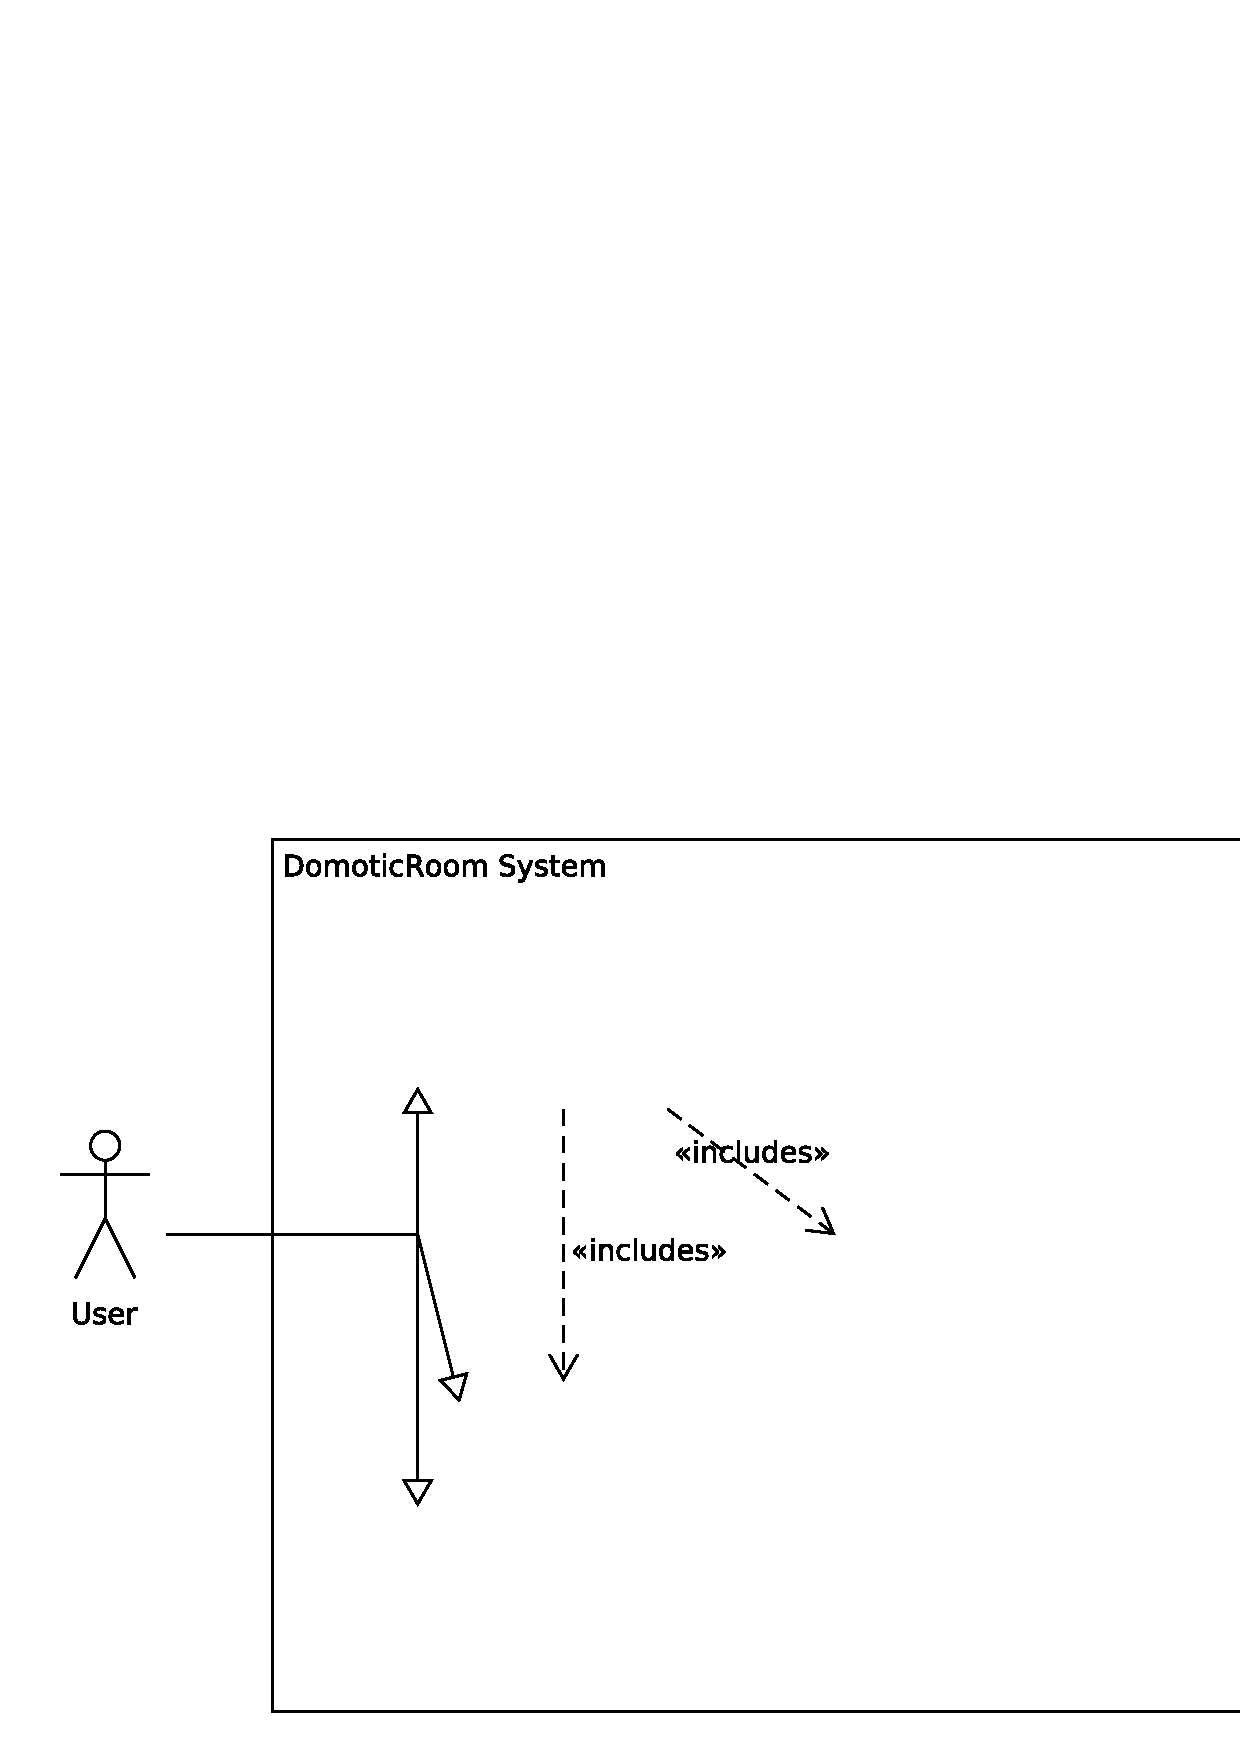
\includegraphics[width=\textwidth]{Figures/UseCases.jpg}
\caption{Casi d'Uso}
\end{figure}

Nell'immagine sopra si possono vedere quali sono le macro operazioni principali effettuate dal sistema e le interazioni con l'esterno. In particolare gli attori che interagiscono con il sistema saranno:

\begin{itemize}
  \item La stanza: con questo attore si intendono i vari parametri che si possono rilevare attraverso i sensori e che quindi saranno di input per il sistema.
  \item Utente: con questo attore rappresenta l'utente che puo' interagire con il sistema.
\end{itemize}

Il sistema \'e stato volutamente suddiviso in tre parti distinte con l'idea di seguire un modello MVC dove per\'o la parte di modello non viene aggiornato attraverso l'input inserito dall'utente, ma direttamente dall'input dei sensori. L'organizzazione hardware ha fortemente influito su questa suddivisione.

\'E inoltre possibile visualizzare le macro operazioni che devono essere effettuate e modellate dal sistema. Si vedano gli scenari di seguito per avere una piu' dettagliata visualizzazione dell'interazione tra le varie parti che lo schema sovrastante vuole rappresentare.


\subsection{Scenario}
\labelssec{Scenarios}


\subsection{Modello del Dominio}

\subsection{Piani di Test}

